\documentclass[11pt,a4paper]{article}
\usepackage[left=2.5cm,right=2.5cm,top=3cm,bottom=3.5cm]{geometry}
\usepackage[ngerman]{babel}
\usepackage[utf8]{inputenc}
\usepackage{graphicx}
\usepackage{amsfonts} 
\usepackage{svg}
\usepackage{amsmath}
\usepackage[rightcaption]{sidecap}
\begin{document}
 
 \begin{center}
  {\scshape\LARGE Grundpraktikum I \par}
  \vspace{1cm}
  {\scshape\Large Versuchsprotokoll\par}
  \vspace{1.5cm}
  {\huge\bfseries Gammaspektroskopie\par}
  \vspace{2cm}
     {\large \itshape{Clemens Schumann, Tassilo Scheffler}\/ \par}
  \vspace{0.5cm}
  {clemensrubenschumann@googlemail.com, \\ tassilo@glief.de}
  \vfill
  betreut von\par
  \textsc{Nele Stetzuhn }
  \vfill
  {\Large 15.03.2018}
 
 \end{center}
 
 \thispagestyle{empty}
 
 \newpage
 \setcounter{page}{1}
 \tableofcontents
 \newpage
 \section*{Gammaspektroskopie}
 \section{\underline{Einleitung}}
 In diesen Versuchen wollen wir 
\section{\underline{Physikalische Grundlagen}}
Atomkerne bestehen aus Protonen und Neutronen. Jeder Atomkern ist über die Anzahl
dieser definiert. Das heißt jedes Nuklid $X$ ist mit $^A_Z{X}$ definiert. $A$ ist dabei
die Massenzahl und $Z$ die Ordnungszahl. Dabei gilt für Protonen $p:~^1_1p$ und für
Neutronen $n:~^1_0n$. Diese Kerne können radioaktiv zerfallen, wenn sie instabil
sind. Dabei gibt es verschiedene Arten des Zerfalls:
\\\\
1. \alpha~- Zerfall: Ein doppelt positiv geladener Heliumkern wird emittiert.
\begin{equation}
    ^A_Z{X} \rightarrow~^{A-4}_{Z-2}Y
\end{equation}
2a. $\beta ^+$ - Zerfall: Ein Proton wandelt sich in ein Neutron, ein Positron und ein
Neutrino um. Das Positron wird anschließend emittiert.
\begin{align}
  p \rightarrow~n + e^+ + \upsilon \\
    ^A_ZX \rightarrow~{^A_{Z-1}Y} + e^+ + \upsilon
\end{align}
2b. $\beta ^-$ - Zerfall: Ein Neutron wandelt sich in ein Proton, ein Elektron und ein
Antineutrino um. Das Elektron wird anschließend emittiert.
\begin{align}
  n \rightarrow~p + e^- + \overline{\upsilon} \\
    ^A_ZX \rightarrow~{^A_{Z+1}Y} + e^- + \overline{\upsilon}
\end{align}
3. $\gamma$ - Zerfall: Hierbei werden $\gamma$ - Quanten emittiert. Das heißt, dass sich nur das Energieniveau des Atoms ändert:
\begin{equation}
    ^A_ZX^* \rightarrow~{^A_ZX} + \gamma
\end{equation}
Die Energie des $\gamma$ - Quants kann mit
\begin{equation}
  E = h \cdot \frac{c}{\lambda}
\end{equation}
berechnet werden. $h$ ist dabei das Planksche Wirkunsquantum, $c$ die
Lichtgeschwindigkeit und $\lambda$ die Wellenlänge des $\gamma$ - Quants.
Der Strahlungsnachweis erfolgt mithilfe eines Geiger-Müller-Zählrohrs. Dieses kann
$\beta^-$ - Strahlung und $\gamma$ - Strahlung messen, indem die Atome des Gases des
Zählrohrs durch das Eintreten der radioaktiven Atome ionisiert werden. Dadurch kommt
es zu einer Elektronenlawine und schließlich zu einem Stromstoß. Daher kann man
mithilfe dessen auch keine zwei exakt aufeinanderfolgende radioaktive Teilchen messen.
Für die Intensität der $\gamma$ - Strahlung gilt
\begin{equation}
  I = I_0e^{- \mu x}
\end{equation}
sobald man annimmt, dass die Wechselwirkungswahrscheinlichkeit der durchstrahlten
Schichtdicke $dx$ proportional ist und dass ein Strahlungsquant bei der Wechsewirkung
mit dem Strahlungsfeld verloren geht. $\mu$ bezeichnet hier den
Absorptionskoeffizient. Bei konstanter Energie ist $\frac{\mu}{\rho}$ mit der Dichte
$\rho$ nahezu konstant.

Bei der Interaktion mit Materie gibt es 3 wesentliche Effekte, die zutreffen können.
\\\\
1. Der Photoeffekt \\
Bei diesem Effekt interagiert ein \gamma~- Quant mit einem Atom. Das \gamma~-
Quant gibt dabei seine gesamte Energie an ein Elektron ab, welches damit aus dem Atom
"geschossen" wird. Dadurch verschwindet das Photon und das Atom hat ein Elektron
weniger.
\\\\
2. Der Compton - Effekt \\
Hierbei interagiert ein \gamma~- Quant mit einem freien Elektron. Da ein Photon ein
Teilchen mit einer relativen Masse hat, hat es auch einen Impuls, welcher an das
Elektron weitergegeben wird. Somit gibt es ein Energiequant an das Elektron ab. Das
Elektron hat damit eine höhere Energie und das Photon eine niedrigere
Bewegungsfrequenz.
\\\\
3. Die Paarerzeugung \\
bei der Paarerzeugung interagiert das \gamma~- Quant mit einem Kern. Wichtig dabei
ist, dass sich ein Photon in der Nähe des Coulomb-Feldes eines Atomkerns in ein
Elektron und ein Positron umwandeln kann und andersherum. Wenn nun Positron und
Elektron aufeinander treffen, so entsteht ein Photon, also ein \gamma~- Quant.
\newpage
\section{\underline{Messprotokoll}}
\section{Aufgaben}
\subsection{} 
Messung  der natürlichen Äquivalentdosisleisung und der Dosisleisung 
des $^{60}Co$-Präparates in 0.5 m Abstand mit einem integrierten Äquivalentdosisleistungsmessgerätes.
Umrechnung auf die Äquivalentdosiswerte pro Jahr in Sv/a und mrem/a.
\subsection{} 
Aufnahme der $\gamma$ - Spektren von $^{60}Co, ^{137}Cs, ^{22}Na$ und $^{241}Am$ und Kalibrierung
des Spektrometers (Kalibrierkurve).
\subsection{}
Bestimmung der Energie der $e^+-e^-$ Vernichtungsstrahlung und Vergleich 
mit der Einsteinschen Beziehung ($E=mc^2$).
\subsection{}
Bestimmung des Auflösungsvermögens des Spektrometers für die $\gamma$-Linie von $^{137}Cs$.
\subsection{}
Bestimmung der maximalen Übertragsenergie beim Compton-Streuprozess (Compton-Kante)
für die $\gamma$-Linie von $^{137}Cs$ und Vergleich mit dem theoretischen Wert aus der Streuformel.
\subsection{}
Überprüfung des Absorptionsgesetzes und Bestimmung der Schwächungskoeffizienten
und Halbwertsdicken für Eisen und Blei für die 0.662 MeV-$\gamma$-Strahlung von $^{137}Cs$.


\section{Geräte}
- Szintillationsdetektor mit Sekundärelektronenvervielfacher und Vorverstärker
\\- Hochspannungs-Netzgerät 
\\- AD-Wandler
\\- Netzgerät
\\- PC mit Monitor und Tastatur
\\- Präparatesatz Co-60, Cs-137, Na-22, Am-241
\\- 2 Sätze Absorber (Pb, Fe) verschiedener Dicke
\\- Präparatehalter mit Pb-Abschirmung
\\- Absorbehalter
\\- Dosisleistungsmessgerät

\section{Skizze}
\subsection{Szintillationsdetektor}
\begin{figure}[htbp] 
  \centering
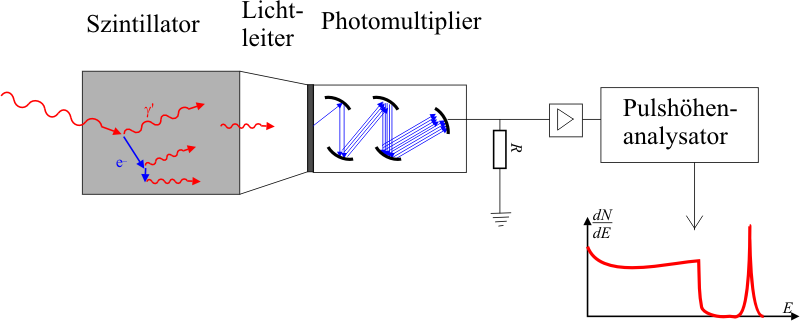
\includegraphics[width=0.7\textwidth]{Szint.jpg}
  \caption{Szintillationsdetektor}
  \label{fig:Bild1}
\end{figure}

\section{Durchführung}
Für Aufgabe 1 misst man mithilfe des Dosisleistungsmessgerätes in der Luft und 
mit 0.5m Abstand zu dem Co-Präparat. \\
Bei Aufgabe 2 benötigt man den PC und idas Tool "measure" auf diesem.
Mithilfe des Netzgerätes und des AD-Wandlers wird dieser dann mit dem Szintillationsdetektor 
mit den verschiedenen Präparaten darin verbunden.
Zwischen Präparat und Detektor sollte möglichst wenig Platz sein.
Schließlich startet man eine Messung auf dem PC und wartet 5 min bis der Graph komplettiert ist. 
Zu beachten ist, dass Na einen Vernichtungspeak und einen Photopeak hat und Co zwei Photopeaks hat. 
Von Beim Am-Präparat wird nur der Photopeak von 0.060 MeV betrachtet, da nur dieser über den Graphen ersichtlich ist.
\\Die Vernichtungsstrahlung von Aufgabe 3 kann bei Natrium betrachtet werden und ausgewertet werden.
Dabei ist die Energie $E=mc^2$ zu beachten.
\\Aufgabe 4 wird gelöst indem man die Standardabweichung betrachtet und diese umrechnet.
\\Für Aufgabe 5 ist das Caesium-Präparat zu betrachten. Die Compton Kante ist 
in dem Graphen recht gut erkennbar. Dabei wird der Mittelwert von Comtpon Kante und keine Compton Kante genommen. 
Der Vergleichswert wird der Streuformel entnommen.
\\Für Aufgabe 6 wird das Absorptionsgesetz genommen und zwischen Cs-Präparat und Detektor 
Blei bzw. Eisen positioniert. Eisen wird in 5 mm Schritten bis 45 mm dazwischen gemessen und jeweils die Anzahl 
der Impulse, die in den Kanälen des Peaks ankommen gemessen. Das selbe wird mit Blei in 3 mm Abständen gemacht.
\section{\underline{Aufbau}}
\newpage
\section{\underline{Auswertung}}
\newpage
\section{\underline{Diskussion}}
\newpage
\section{\underline{Messwerte}}
 \end{document}
